\documentclass[12pt,a4paper,final]{article} %draft

\usepackage[english, russian]{babel}

\usepackage[final]{pdfpages}

\usepackage{textcomp,enumitem}

\usepackage{amsmath,amsthm,amssymb}

\usepackage{fancyhdr}

\usepackage{upgreek}

\usepackage{tipa}

\usepackage{tikz}

\usepackage{graphicx}

\usepackage{pgfplots}

\usepackage{indentfirst}

\usepackage{gensymb}

\usepackage{amssymb}

%usepackage{pdfpages}

\usepackage[unicode, pdftex, colorlinks, urlcolor=blue]{hyperref}

\usepackage[T2A]{fontenc}

\usepackage[utf8]{inputenc}

\usepackage[left=2cm,right=2cm,top=2cm,bottom=2cm,bindingo ffset=0cm]{geometry}

\usepackage{graphics}

\renewcommand{\arraystretch}{1.5}

\linespread{1.5}

\pagestyle{plain}

\usepackage{hyperref}

\usepackage{xcolor}

\definecolor{keywords}{RGB}{0,0,255}
\definecolor{comments}{RGB}{0,128,0}
\definecolor{strings}{RGB}{255,0,90}
\definecolor{lightbeige}{RGB}{255,240,220} % светло-бежевый цвет


\usepackage{listings}

\lstset{
	language=SQL, % Язык программирования
	captionpos=t, % Позиция подписи (b - внизу)
	frame=single, % устанавливаем рамку для всего листинга
	framesep=3pt, % отступ рамки от текста
	%xleftmargin=0mm, % Отступ слева
	%frame=lines, % Тип рамки (single - одинарная, double - двойная, lines - линии)
	framerule=0.25mm, % Толщина рамки
	% backgroundcolor=\color{lightbeige}, % устанавливаем цвет фона
	literate=
	{а}{{\selectfont\char224}}1
	{б}{{\selectfont\char225}}1
	{в}{{\selectfont\char226}}1
	{г}{{\selectfont\char227}}1
	{д}{{\selectfont\char228}}1
	{е}{{\selectfont\char229}}1
	{ж}{{\selectfont\char230}}1
	{з}{{\selectfont\char231}}1
	{и}{{\selectfont\char232}}1
	{й}{{\selectfont\char233}}1
	{к}{{\selectfont\char234}}1
	{л}{{\selectfont\char235}}1
	{м}{{\selectfont\char236}}1
	{н}{{\selectfont\char237}}1
	{о}{{\selectfont\char238}}1
	{п}{{\selectfont\char239}}1
	{р}{{\selectfont\char240}}1
	{с}{{\selectfont\char241}}1
	{т}{{\selectfont\char242}}1
	{у}{{\selectfont\char243}}1
	{ф}{{\selectfont\char244}}1
	{х}{{\selectfont\char245}}1
	{ц}{{\selectfont\char246}}1
	{ч}{{\selectfont\char247}}1
	{ш}{{\selectfont\char248}}1
	{щ}{{\selectfont\char249}}1
	{ъ}{{\selectfont\char250}}1
	{ы}{{\selectfont\char251}}1
	{ь}{{\selectfont\char252}}1
	{э}{{\selectfont\char253}}1
	{ю}{{\selectfont\char254}}1
	{я}{{\selectfont\char255}}1
	{А}{{\selectfont\char192}}1
	{Б}{{\selectfont\char193}}1
	{В}{{\selectfont\char194}}1
	{Г}{{\selectfont\char195}}1
	{Д}{{\selectfont\char196}}1
	{Е}{{\selectfont\char197}}1
	{Ж}{{\selectfont\char198}}1
	{З}{{\selectfont\char199}}1
	{И}{{\selectfont\char200}}1
	{Й}{{\selectfont\char201}}1
	{К}{{\selectfont\char202}}1
	{Л}{{\selectfont\char203}}1
	{М}{{\selectfont\char204}}1
	{Н}{{\selectfont\char205}}1
	{О}{{\selectfont\char206}}1
	{П}{{\selectfont\char207}}1
	{Р}{{\selectfont\char208}}1
	{С}{{\selectfont\char209}}1
	{Т}{{\selectfont\char210}}1
	{У}{{\selectfont\char211}}1
	{Ф}{{\selectfont\char212}}1
	{Х}{{\selectfont\char213}}1
	{Ц}{{\selectfont\char214}}1
	{Ч}{{\selectfont\char215}}1
	{Ш}{{\selectfont\char216}}1
	{Щ}{{\selectfont\char217}}1
	{Ъ}{{\selectfont\char218}}1
	{Ы}{{\selectfont\char219}}1
	{Ь}{{\selectfont\char220}}1
	{Э}{{\selectfont\char221}}1
	{Ю}{{\selectfont\char222}}1
	{Я}{{\selectfont\char223}}1,
	numbers=left, % пронумеровать строки с левой стороны
	breaklines=true % разрешает автоматический перенос строк
	basicstyle=\small\ttfamily\color{black}, % устанавливаем межстрочный интервал, размер шрифта и цвет текста
	aboveskip=0pt, % Устанавливаем отступ перед строкой в ноль
	belowskip=0pt, % Устанавливаем отступ после строки в ноль
	keywordstyle=\color{keywords},
	commentstyle=\color{comments},
	stringstyle=\color{strings},
	keywords={SELECT, DISTINCT, JOIN, ON, WHERE, FROM, AS, AND, OR, HAVING, COUNT, GROUP, BY, IN}, % Добавляем нужные ключевые слова
}


\usepackage{moreverb} 


\setlist[enumerate,itemize]{leftmargin=1.2cm, itemsep=12pt , parsep=0pt} %отступ в перечислениях

\hypersetup{colorlinks,
	allcolors=[RGB]{0 0 255}}

\lstloadlanguages{ [LaTeX] TeX}

%\lstset{language =[LaTeX] TeX, 
	%extendedchars=true , 
	%escapechar = | , 
	%frame=tb , 
	%commentstyle=\itshape , 
	%stringstyle =\bfseries}

\textheight=24cm 
\textwidth=16cm
\oddsidemargin=0pt 
\topmargin=-1.5cm
\parindent=24pt 
\parskip=0pt 
\tolerance=2000 
\flushbottom 

%\usepackage[font=scriptsize]{caption}
\usepackage[labelsep=period]{caption}



\begin{document}
	\thispagestyle{empty}
	\begin{center}
		\vspace{36pt}
		{\Large МИНОБРНАУКИ РОССИИ }\\
		\vspace{24pt}
		{\large ФЕДЕРАЛЬНОЕ ГОСУДАРСТВЕННОЕ БЮДЖЕТНОЕ ОБРАЗОВАТЕЛЬНОЕ УЧРЕЖДЕНИЕ ВЫСШЕГО ПРОФЕССИОНАЛЬНОГО ОБРАЗОВАНИЯ}\\
		\vspace{24pt}
		{\Large \bf <<САНКТ-ПЕТЕРБУРГСКИЙ ПОЛИТЕХНИЧЕСКИЙ УНИВЕРСИТЕТ ПЕТРА ВЕЛИКОГО>>}\\
		\vspace{24pt}
		{\large Институт Компьютерных наук и кибербезопасности}\\
		{\large Высшая школа технологий искусственного интеллекта}\\
		{\large Направление 02.03.01 Математика и компьютерные науки}\\
		\vspace{36pt}
		{\Large ОТЧЁТ ПО КУРСОВОЙ РАБОТЕ}\\
		\vspace{12pt}
		{\large по дисциплине <<Проектирование WEB приложений>>}\\
		\vspace{24pt}
		{\large Проектирование приложения по предметной области <<Спортивная школа олимпийского резерва по спортивной акробатике>>}\\
	\end{center}
	\vspace{48pt}
	{\large Студент: \hspace{6.6cm} \underline{\hspace{3.5cm}} Плужникова Ю.С.}\\
	{\large Преподаватель: \hspace{5cm} \underline{\hspace{3.5cm}} Попов С.Г.}\\
	\vspace{24pt}
	\begin{flushright}
		«\underline{\hspace{1cm}}»\underline{\hspace{3cm}}20\underline{\hspace{0.7cm}}г.
	\end{flushright}
	\vspace{40pt}
	\begin{center}
		{\large Санкт-Петербург, 2025}
	\end{center}
	
	
	\newpage
	\tableofcontents
	
	\newpage
\section{Постановка задачи}
\par Данная курсовая работа состоит из трех частей:

\begin{enumerate}
	\item Аналитика
	\par В первой части работы необходимо:
	\begin{enumerate}
		\item Выбрать фрагмент текста из описания предметной области курсовой работы по дисциплине <<Теоретические основы баз данных>>;
		\item Отредактировать выбранный фрагмент текста;
		\item Максимально полно нарисовать ER-диаграмму по выбранному тексту и описать её;
		\item Расширить описание предметной области: описать процессы.
	\end{enumerate}
	\item USE-CASE
	\par Во второй части работы необходимо:
		\begin{enumerate}
		\item Декомпозировать основной и вспомогательные процессы на несколько дочерних;
		\item Для основного и дочерних процессов составить use-case диаграммы;
		\item Составить словесное описание каждой use-case диаграммы.
	\end{enumerate}
\end{enumerate}
	
	\newpage
	\section{Аналитика}
\subsection{Выбранный фрагмент текста}
\par На \hyperref[fig:im1]{рисунке 1} представлен выбранный фрагмент текста из описания предметной области.
\begin{figure}[htbp]
	\centering
	\fbox{\parbox{1.0\textwidth}{Для того чтобы подготовить спортсмена-профессионала в данном виде спорта, обучение в подобных школах ведется ни один год. По каждому спортсмену ведется личное дело, в котором фиксируются его разряд, его достижения, победы, участия в различных соревнованиях. Помимо этого, спортивная акробатика – сложно-координационный вид спорта, а значит очень важно следить за здоровьем спортсменов. Диспансеризация проходит раз в полгода, по результатам которой решается, допускается ли спортсмен к тренировкам и соревнованиям. Данные о медосмотрах также записываются в личное дело – зачетную книжку. Лучшие спортсмены, которые имеют разряд КМС и выше, могут попасть в сборную края (области).Также ведется журнал учета количества свободных мест у каждого тренера. При поступлении в спортивную школу можно выбрать тренера на основе его категории, стажа работы, звания, образования, наград, наличия свободных мест. Также имеется возможность посмотреть перечень известных спортсменов, которых выпустил тренер.}}
	\caption{Выбранный фрагмент текста из описания предметной области}
	\label{fig:im1}
\end{figure}

\subsection{Отредактированный фрагмент текста №1}
\par На \hyperref[fig:im2]{рисунке 2} представлен отредактированный фрагмент текста.
\begin{figure}[htbp]
	\centering
	\fbox{\parbox{1.0\textwidth}{Администратор спортивной школы ведет журнал учета, который дает выбор тренера на основе его категории, стажа работы, звания, образования, наград, наличия свободных мест. Тренер обучает спортсменов, которые владеют своим личным делом - зачетной книжкой. Зачетная книжка содержит соревнования, в которых участвует спортмен. Каждое соревнование масштабируется статусом и имеет свое  название, дату и место проведения. Также спортсмен выполняет разряды, которые фиксируются в его зачетной книжке. Лучшие спортсмены, имеющие разряд КМС и выше, могут попасть в сборную края, отбор в которую проводят специальные члены отборочной комиссии. Спортсмены регулярно проходят диспансеризации, которые характеризуются датой прохождения и результатом прохождения - допуском к тренировкам и соревнованиям. Медицинские работники проводят диспансеризации, которые записываются в зачетные книжки спортсменов.}}
	\caption{Отредактированный фрагмент текста №1}
	\label{fig:im2}
\end{figure}

\subsection{Отредактированный фрагмент текста №2}
\par На \hyperref[fig:im2]{рисунке 3} представлен отредактированный фрагмент текста №1.
\begin{figure}[htbp]
	\centering
	\fbox{\parbox{1.0\textwidth}{Родитель поступающего ребенка обращается к администратору спортивной школы. Администратор предоставляет родителю возможность выбора тренера на основе его категории, стажа работы, звания, образования, наград и наличия свободных мест. Выбор родителя фиксируется в журнале учета, который ведет администратор. Администратор назначает дату прохождения индивидуального отбора поступающего ребенка. Индивидуальный отбор проводит тренер. Тренер записывает результаты отбора в специальный протокол. По результатам отбора тренер принимает решение о приеме или отказе поступающего ребенка. Администратор дает родителю список документов. Родитель формирует комплект документов по этому списку. Родитель заполняет заявление на зачисление поступающего ребенка в спортивную школу. Родитель предоставляет комплект документов администратору.}}
	\caption{Отредактированный фрагмент текста №2}
	\label{fig:im3}
\end{figure}

\newpage
\subsection{ER-диаграмма и ее описание}
\par ER-диаграмма представлена на \href{er.pdf}{рисунке 4}
\par Родитель поступающего ребенка обращается к администратору. Администратор предоставляет родителю возможность выбора тренера на основе его категории, стажа работы, звания, образования, наград и наличия свободных мест. Выбор родителя фиксируется в журнале учета, который ведет администратор. Администратор назначает дату прохождения индивидуального отбора поступающего ребенка. Индивидуальный отбор проводит тренер. Тренер записывает результаты отбора в протокол. По результатам отбора тренер принимает решение о приеме или отказе поступающего ребенка. Администратор дает родителю список документов. Родитель формирует комплект документов по этому списку. Родитель заполняет заявление на зачисление поступающего ребенка. Родитель предоставляет комплект документов администратору.
\newpage
\includepdf[pages=-,fitpaper]{er.pdf} 
\setcounter{figure}{4}

\subsection{Описание процессов}
\subsubsection{Основной процесс}
\par \textbf{Основной процесс} - обучение спортсменов. 
\par Перед началом тренировочного сезона тренеры формируют списки своих групп и составляют расписание учебно-тренировочных занятий в соответствии с режимом работы спортивной школы и нормативным документам. Расписание занятий утверждается директором учреждения. 
\par Каждое занятие состоит из разминки, растяжки, основной части, включающей выполнение и изучение упражнений и технических элементов, и завершающей части, направленной на подкачку и повторную растяжку. Несколько раз в неделю проводится дополнительная часть, называемая хореографией. В ходе тренировочного сезона тренер ведет статистику посещаемости спортсменов, которую передает администрации спортшколы. Спортсмены упорно тренируются, участвуют в соревнованиях, выполняют разряды и проходят медицинские обследования. 
\par В конце тренировочного сезона - в период летних каникул - организуется выезд на тренировочные сборы, где в течение 3-х недель непрерывно тренируются и выполняют контрольные нормативы, находясь в своей лучшей спортивной форме. Результаты нормативов тренер записывает в протокол и проводит анализ с результатами предыдущего года. Обучающиеся, выполнившие требования контрольно-переводных нормативов, переводятся на следующий год. Лица, не выполнившие требования контрольно-переводных нормативов, решением
педагогического совета учреждения могут быть оставлены на предыдущем
этапе спортивной подготовки или переведены в группы общей физической подготовки на платной основе. Обучающиеся, заболевшие в период промежуточной аттестации, могут быть освобождены от неё на основании справки из медицинского учреждения. В случае отъезда обучающегося в отпуск с родителями до окончания периода промежуточной аттестации, он имеет право пройти досрочную промежуточную аттестацию на основании заявления родителей (законных представителей) по согласованию с тренером-преподавателем.  
\par По окончании сборов спортсменам дается 3 недели отдыха, после чего они снова приступают к тренировкам и готовятся к началу нового тренировочного сезона. 
\par Обучение спортсменов длится до достижения ими 18 лет, после чего они официально выпускаются из спортивной школы. Администрация школы проводит награждение и выдает свидетельство об окончании спортшколы. После этого спортсмен может продолжить тренировочный процесс по своему желанию.

\subsubsection{Вспомогательные процессы}
\par \textbf{Прием граждан в спортивную школу:} 
\par Родители или законные представители ребенка обращаются к администратору спортивной школы. Администратор запрашивает основную информацию о ребенке, такую как его ФИО, дата рождения, наличие предыдущего спортивного опыта. Далее администратор проверяет журнал учета на наличие свободных мест в группах тренеров. Если свободные места имеются, администратор назначает дату индивидуального отбора.  Если нет - администратор предлагает родителям оставить заявку в листе ожидания. В назначенный день родитель вместе с ребенком приходит на этот отбор, который проводит тренер. Индивидуальный отбор проводится в целях выявления у поступающих физических, психологических способностей и (или) двигательных умений, необходимых для освоения дополнительных образовательных программ спортивной подготовки по спортивной акробатике. На основании результатов отбора тренер принимает решение о приеме поступающего к себе в группу. Результаты отбора и свое решение тренер заносит в протокол и передает администратору. В случае положительного решения тренера администратор запрашивает родителя заполнить заявление на зачисление в спортшколу.  Иначе - родители поступающих вправе подать апелляцию по процедуре и (или) результатам проведения индивидуального отбора в апелляционную комиссию не позднее следующего рабочего дня после объявления результатов индивидуального отбора. При подаче заявления родителем поступающего предоставляются следующие документы: копия свидетельства о рождении поступающего; медицинские документы, подтверждающие отсутствие у поступающего противопоказаний для освоения дополнительной образовательной программы спортивной подготовки (медицинская справка от терапевта поликлиники по месту жительства о возможности занятий ребенка в спортивной секции); фотография ребенка 3 х 4 см – 1 штука; анкета обучающегося. Заполненное заявление и собранные документы администратор передает приемочной комиссии учреждения. На каждого поступающего заводится личное дело, в котором хранятся все
сданные документы и материалы результатов индивидуального отбора.
Личные дела поступающих хранятся в учреждении не менее трех месяцев с
начала объявления приёма в учреждение. Если приемочная комиссия утверждает зачисление, директор учреждения оформляет приказ о зачислении. Администратор вносит данные в журнал учета спортивной школы и уведомляет родителя о принятом решении. В случае отказа комиссия предоставляет родителю обоснование отказа. \\

\par \textbf{Прохождение диспансеризации:}
\par Процесс прохождения диспансеризации организуется медицинскими работниками врачебно-физкультурного диспансера в соответствии с установленным графиком. Заместитель директора по учебно-спортивной работе спортивной школы совместно с заместителем главного врача диспансера согласует даты диспансеризации для каждой группы спортсменов и уведомляет тренеров о предстоящем медицинском обследовании. Тренеры передают информацию своим спортсменам и их родителям. В назначенный день спортсмены прибывают в диспансер. Регистратор выдает каждому спортсмену его медицинскую карту в случае ее наличия, либо спортсмен заполняет заявления, указывая в них свои данные и согласия. Сначала спортсмен отправляется к врачу-терапевту, который проводит общий осмотр, измеряет рост, вес, давление и оценивает общее физическое состояние спортсмена. Затем терапевт выдает список кабинетов врачей, которые должен посетить спортсмен. Спортсмен проходит комплексное медицинское обследование по этому списку и возвращается в кабинет терапевта, который по результатам обследования принимает решение о выдаче допуска спортсмена к учебно-образовательному процессу и соревнованиям. В случае положительного решения терапевт ставит печать в зачетную книжку спортсмена, которая свидельствует о наличии допуска. В случае выявления у спортсмена противопоказаний для занятий спортом врач может выдать временный или постоянный отвод. Спортсмен с временным отводом обязан пройти повторное обследование в установленный срок. Спортсмен с постоянным отводом исключается из учебно-тренировочного процесса и при наличии желания переводится в группы оздоровительной физической культуры. Если спортсмен пропускает диспансеризацию без уважительной причины, его тренер вправе не допускать его к тренировкам до прохождения обследования. \\

\par \textbf{Отбор спортсменов в сборную края:} 
\par Процесс отбора спортсменов в сборную края проходит под руководством отборочной комиссии, состоящей из представителей комитета по физической культуре и спорту. Отборочная комиссия определяет критерии включения в сборную, которые включают возрастные ограничения, минимальный спортивный разряд (обычно КМС и выше), достижения на соревнованиях определенного уровня (региональные, всероссийские, международные). Заместитель директора по учебно-спортивной работе получает уведомление о начале отбора и поручает тренерам подготовить списки кандидатов. В этих списках указываются: ФИО спортсменов, их возраст, разряд, основные спортивные достижения за последний год, а также состояние здоровья (или собирают зачетные книжки спортсменов, где есть вся эта информация). Затем готовые списки передаются заместителю директора по учебно-спортивной работе, который проверяет их на соответствие требованиям и направляет документы в отборочную комиссию. Секретарь комиссии принимает и передает документы другим членам. Они проверяют соответствие кандидатов установленным критериям и формируют список сборной. Спортсмены, вошедшие в этот список, включаются в состав сборной, что фиксируется приказом от руководителя комитета по физической культуре и спорту. Если спортсмен не включен в сборную, он может продолжить тренировки для повторного участия в отборе на следующий год. В случае возникновения спорных ситуаций тренер имеет право подать апелляцию, приложив дополнительные аргументы в пользу своего воспитанника. Если количество мест в сборной ограничено, спортсмен, не прошедший отбор, может быть оставлен в резервном списке на случай необходимости замены основных участников.\\

\par \textbf{Организация соревнований:} \\
\par Процесс начинается с определения статуса соревнования, его названия, места и даты проведения, что осуществляет директор спортшколы, которая организует данное мероприятие. Затем администратор подготавливает объявление о соревновании и публикует его на официальном сайте спортивной школы и в социальных сетях. Если соревнование открыто для участия других спортивных школ, администратор дополнительно рассылает приглашения. Далее тренеры подают заявки на участие своих спортсменов, указывая их ФИО, возраст, спортивный разряд, составы, а также прикрепляют медицинские допуски спортсменов. Администратор принимает заявки, проверяет их соответствие требованиям и передает данные документоведу, который формирует общий список участников и распределяет их по категориям. После этого заместитель директора по учебно-спортивной работе назначает главных судей, технических судей, секретарей и медицинских работников. Заместитель директора по административно-хозяйственной части заказывает наградные материалы — медали, грамоты, кубки и сертификаты. Затем секретарь соревнований составляет расписание проведения соревнования на каждый день, в том числе и на опробование. В день соревнования все работники заранее прибывают на место проведения. Медицинский работник дежурит на площадке для оказания помощи в случае получения спортсменами травм. Спортсмены выступают согласно расписанию. Судьи фиксируют результаты каждого состава в протоколах, выставляя баллы, а секретари обрабатывают данные и ведут учет результатов. По завершении соревнований секретари сверяют протоколы, составляют итоговую таблицу с результатами участников. После этого ведущий церемонии награждения объявляет результаты и вручает медали, грамоты и кубки. Результаты соревнований фиксирует документовед в зачетных книжках спортсменов.\\

\par \textbf{Присвоение спортивных разрядов:}\\
Тренер отслеживает достижения своих спортсменов на официальных соревнованиях и, если спортсмен выполнил норматив для получения нового разряда, подготавливает заявку. В заявке указываются: ФИО спортсмена, дата рождения, спортивная школа, тренер, разряд, на который подается заявка, соревнование(я), на котором был выполнен норматив. К заявке прилагаются копии протоколов соревнований, где зафиксированы результаты спортсмена. Заместитель директора по учебно-спортивной работе проверяет правильность заполнения заявки. Если заявка корректна, она направляется в комитет по физической культуре и спорту. В случае ошибок в заявке на разряд она возвращается тренеру на исправление. Члены спортивного комитета проверяют соответствие поданного результата требованиям разрядных норм, статуса соревнований (разряд может быть присвоен только на официальных соревнованиях, включенных в календарный план). Если все требования соблюдены, заявка утверждается. На основании утвержденных заявок руководитель комитета по спорту выпускает приказ о присвоении разрядов. После выхода приказа документовед спортшколы вносит присвоенный разряд в зачетную книжку спортсмена. При достижении значимых разрядов (КМС, МС) спортсмену выдается удостоверение о спортивном разряде. 

\newpage
\section{USE-CASE}
\subsection{Уровень 1}
\par На \hyperref[fig:im5]{рисунке 5} представлена use-case диаграмма первого уровня.
\begin{figure}[h!]
	\centering
	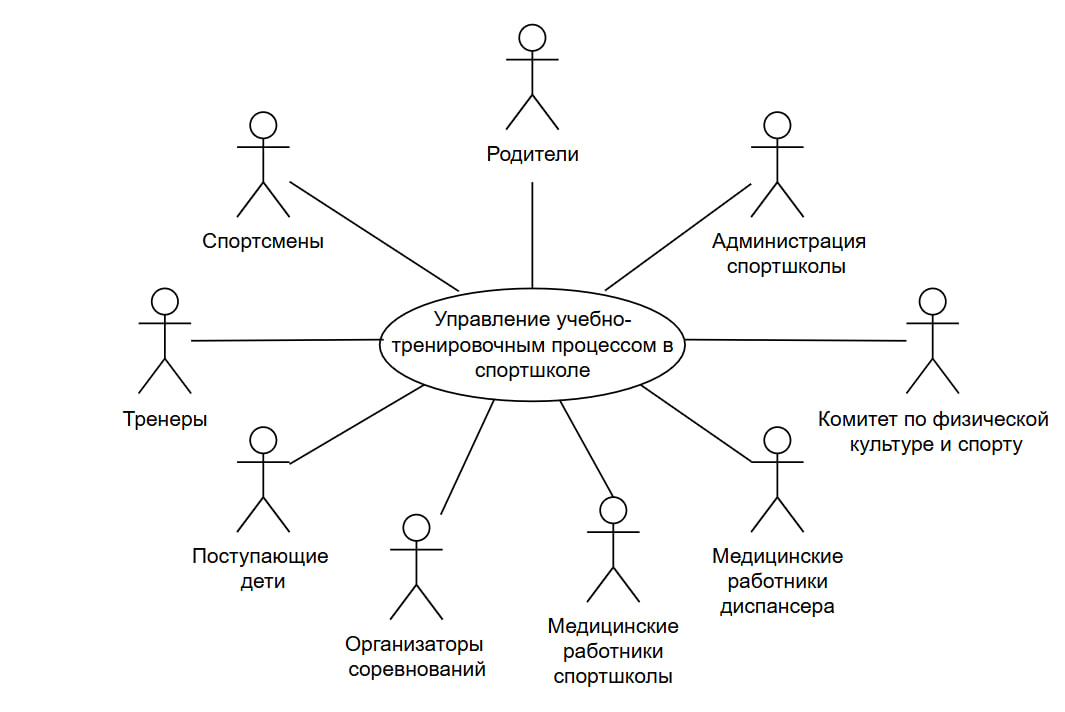
\includegraphics[width=1.0\linewidth]{images/2}
	\caption{Use-case диграмма основного процесса}
	\label{fig:im5}
\end{figure}	

\par \textbf{Акторы:} Спортсмены, тренеры, поступающие дети, родители, медицинские работники спортшколы, администрация спортшколы, организаторы соревнований, комитет по физической культуре и спорту, медицинские работники диспансера.

\par \textbf{Триггер:} Начало учебно-тренировочного сезона.

\par \textbf{Входные данные:} Объявление о наборе детей в спотшколу, желание родителей записать детей в спортивную школу, желание спортсменов тренироваться и участвовать в соревнованиях, наличие свободных мест в группах, медицинские допуски спортсменов.

\par \textbf{Выходные данные:} Спортсмены получают спортивную подготовку, разряды и награды на соревнованиях, выпуск спортсменов из спортивной школы.

\par \textbf{Основной процесс:}
\begin{enumerate}[nosep, label=1.\arabic*]   
	\item Набор детей в спортшколу.
	\item Организация медицинского обследования.
	\item Проведение тренировок.
	\item Участие в соревнованиях.
	\item Присвоение спортивных разрядов.
	\item Отбор в сборную.
	\item Проведение промежуточной аттестации.
	\item Проведение тренировочных сборов.
	\item Выпуск совершеннолетних спортсменов.
	\item Переход к п. 1.
\end{enumerate}

\vspace{12pt}
\par \textbf{Декомпозиция use-case первого уровня}

\par \textbf{Основной процесс:}
\begin{enumerate}[nosep, label=1.1.\arabic*]  
	\item Родители подают заявки на зачисление детей в спортшколу.
	\item Администрация спортшколы проверяет наличие свободных мест в группах.
	\item Администрация спортшколы уведомляет родителя поступающего ребенка о проведении индивидуального отбора.
	\item Тренер проводит индивидуальный отбор поступающих детей.
	\item Тренер совместно с администрацией школы формирует списки групп.
	\item Администрация спортшколы уведомляет родителей о зачислении детей.
\end{enumerate}
\begin{enumerate}[nosep, label=1.2.\arabic*]  
	\item Администрация спортшколы согласовывает график диспансеризации с работниками диспансера.
	\item Тренер уведомляет спортсменов и их родителей о дате диспансеризации.
	\item Спортсмены проходят медицинское обследование в диспансере.
	\item Медицинские работники диспансера вносят данные о допусках в зачетные книжки спортсменов.
\end{enumerate}
\begin{enumerate}[nosep, label=1.3.\arabic*]
	\item Спортсмены прибывают на тренировку в назначенное время.
	\item Тренер проводит разминку и основные тренировочные упражнения.
	\item Спортсмены выполняют упражнения под руководством тренера.
	\item Тренер корректирует технику выполнения упражнений.
	\item Тренер проводит завершающую часть тренировки (подкачка и растяжка).
	\item Тренер ведет статистику посещаемости спортсменов.
\end{enumerate}
\begin{enumerate}[nosep, label=1.4.\arabic*]  
	\item Тренер подает заявки на участие спортсменов в соревнованиях.
	\item Медицинские работники спортивной школы проверяют допуски спортсменов.
	\item Спортсмены выступают на соревнованиях.
	\item Судьи фиксируют результаты соревнований.
	\item Организаторы соревнований награждают спортсменов.
	\item Администрация спортшколы фиксирует результаты соревнований в зачетных книжках спортсменов.
\end{enumerate}
\begin{enumerate}[nosep, label=1.5.\arabic*]  
	\item Тренер подготавливает заявки на присвоение разрядов.
	\item Администрация спортшколы проверяет заявки.
	\item Администрация спортшколы направляет заявки в комитет по физической культуре и спорту.
	\item Комитет по физической культуре и спорту утверждает разряды.
	\item Администрация спортшколы вносит данные о разрядах в зачетные книжки спортсменов.
\end{enumerate}
\begin{enumerate}[nosep, label=1.6.\arabic*]  
	\item Тренер подготавливает списки кандидатов в сборную.
	\item Администрация спортшколы проверяет списки.
	\item Администрация спортшколы направляет списки в комитет по физической культуре и спорту.
	\item Комитет по физической культуре и спорту формирует список сборной.
	\item Тренер уведомляет спортсменов о включении в сборную.
\end{enumerate}
\begin{enumerate}[nosep, label=1.7.\arabic*]  
	\item Тренер проводит контрольные нормативы у спортсменов.
	\item Тренер фиксирует результаты нормативов.
	\item Администрация спортшколы переводит спортсменов на следующий этап подготовки.
	\item Тренер уведомляет спортсменов о результатах аттестации.
\end{enumerate}
\begin{enumerate}[nosep, label=1.8.\arabic*]  
	\item Администрация спортшколы организует тренировочные сборы.
	\item Тренер проводит тренировки на сборах.
	\item Тренер проводит контрольные нормативы на сборах.
	\item Тренер подводит итоги сборов.
\end{enumerate}
\begin{enumerate}[nosep, label=1.9.\arabic*]  
	\item Тренер подводит итоги достижений спортсменов.
	\item Администрация школы организует церемонию выпуска.
	\item Родители приглашаются на церемонию.
	\item Администрация школы вручает свидетельства об окончании и награды.
	\item Тренер уведомляет выпускников о возможности продолжения тренировок.
\end{enumerate}

\par \textbf{Альтернативный процесс:} \\
1.1.3.1 Администрация спортшколы предлагает родителям оставить заявку в листе ожидания. \\
1.1.6.1 Администрация спортшколы уведомляет родителей об отказе в зачислении с обоснованием своего решения. \\
1.2.4.1 Медицинские работники диспансера выдают временный отвод от тренировок и соревнований. \\
1.2.4.2 Медицинские работники диспансера запрещают спортсмену заниматься спортом - постоянный отвод. \\
1.3.1.1 Пропуск тренировки без уважительной причины. Тогда тренер проводит беседу с родителями. \\
1.3.3.1 Получение травмы. Медицинские работники спортшколы оказывают первую помощь спортсмену.\\
1.4.2.1 Если у спортсмена отсутствует медицинский допуск, администрация спортшколы исключает его из списка участников.\\
1.5.3.1 Если заявка на присвоение разряда заполнена некорректно, администрация спортшколы возвращает ее тренеру на доработку. \\
1.5.4.1 Комитет по физической культуре и спорту уведомляет администрацию спортивной школы о причинах отказа в утверждении разрядов. \\
1.6.3.1 Администрация спортшколы возвращает список тренеру на доработку. \\
1.7.3.1 Администрация спортшколы оставляет спортсменча на предыдущем этапе подготовки. \\
1.7.3.2 Администрация спортшколы назначает спортсмену новую дату аттестации.

\includepdf[pages=-,fitpaper]{us2.pdf} 
\setcounter{figure}{6}

\subsection{Уровень 2}
\subsubsection{Use-case 1.1}
\par На \hyperref[fig:im7]{рисунке 7} представлена use-case диаграмма процесса набора детей в спортшколу.
\begin{figure}[h!]
	\hspace{- 1.55cm} 
	\centering
	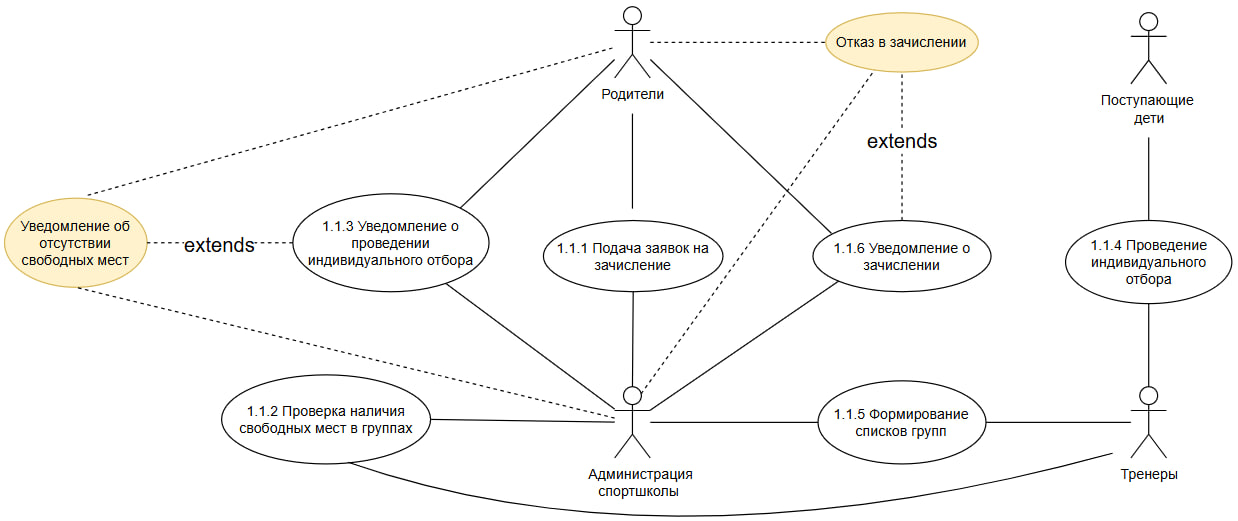
\includegraphics[width=1.1\linewidth]{images/4}
	\caption{Use-case диграмма процесса набора детей в спортшколу}
	\label{fig:im7}
\end{figure}	

\par \textbf{Акторы:} Родители, администрация спортшколы, тренеры, поступающие дети.
\par \textbf{Триггер:} Начало учебно-тренировочного сезона.
\par \textbf{Входные данные:} Объявление о наборе детей в спотшколу, желание родителей записать детей в спортивную школу.
\par \textbf{Выходные данные:} Сформированные списки учебных групп.

\par \textbf{Основной процесс:}
\begin{enumerate}[nosep, label=1.1.\arabic*]
	\item Родители подают заявки на зачисление детей в администрацию спортшколу.
	\item Администрация спортшколы проверяет наличие свободных мест в группах.
	\item Администрация спортшколы уведомляет родителя поступающего ребенка о проведении индивидуального отбора.
	\item Тренер проводит индивидуальный отбор поступающих детей.
	\item Тренер совместно с администрацией школы формирует списки групп.
	\item Администрация спортшколы уведомляет родителей о зачислении детей.
\end{enumerate}

\par \textbf{Альтернативный процесс:} \\
1.1.3.1 Уведомлении об отсутствии свободных мест. Администрация спортшколы предлагает родителям оставить заявку в листе ожидания. \\
1.1.6.1 Отказ в зачислении. Администрация спортшколы уведомляет родителей об отказе в зачислении с обоснованием своего решения. 

\subsubsection{Use-case 1.2}
\par На \hyperref[fig:im8]{рисунке 8} представлена use-case диаграмма процесса организации медицинского обследования. 
\begin{figure}[h!]
	\hspace{- 2cm} 
	\centering
	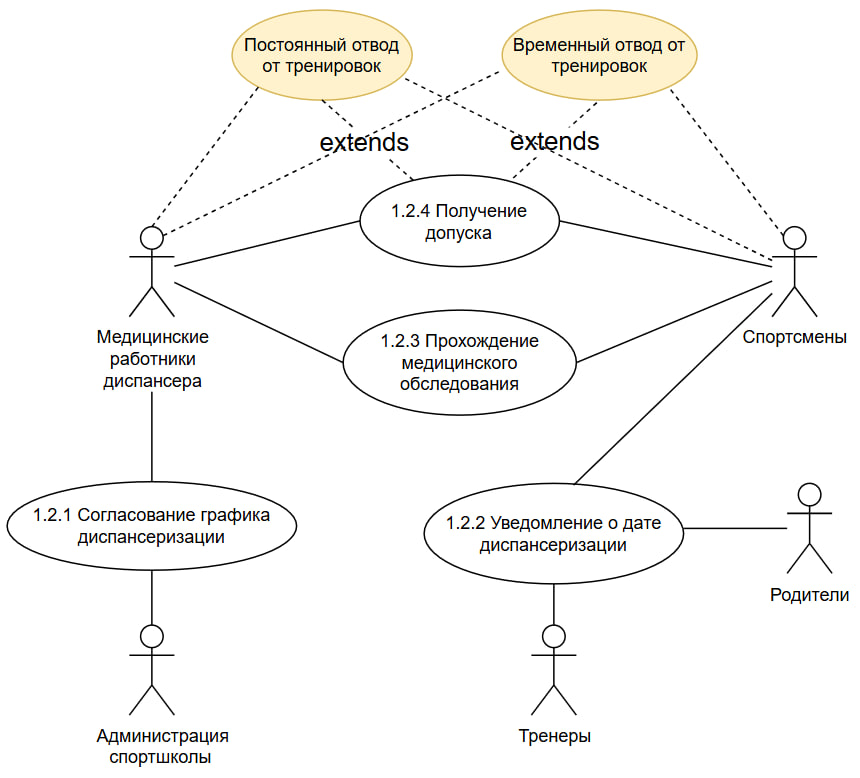
\includegraphics[width=1.1\linewidth]{images/5}
	\caption{Use-case диаграмма процесса организации медицинского обследования}
	\label{fig:im8}
\end{figure}	

\par \textbf{Акторы:} Спортсмены, медицинские работники диспансера, тренеры, администрация спортшколы, родители.
\par \textbf{Триггер:} Начало учебно-тренировочного сезона или истечение срока действия предыдущих медицинских допусков.
\par \textbf{Входные данные:} Медицинские карты спортсменов.
\par \textbf{Выходные данные:} Медицинские допуски спортсменов, постоянные или временные отводы от тренировок.

\par \textbf{Основной процесс:}
\begin{enumerate}[nosep, label=1.2.\arabic*]  
	\item Администрация спортшколы согласовывает график диспансеризации с работниками диспансера.
	\item Тренер уведомляет спортсменов и их родителей о дате диспансеризации.
	\item Спортсмены проходят медицинское обследование в диспансере.
	\item Медицинские работники диспансера вносят данные о допусках в зачетные книжки спортсменов.
\end{enumerate}

\par \textbf{Альтернативный процесс:} \\
1.2.4.1 Медицинские работники диспансера выдают временный отвод от тренировок и соревнований. \\
1.2.4.2 Медицинские работники диспансера запрещают спортсмену заниматься спортом - постоянный отвод.

\subsubsection{Use-case 1.3}
\par На \hyperref[fig:im9]{рисунке 9} представлена use-case диаграмма процесса проведения тренировок. 
\begin{figure}[h!]
	\centering
	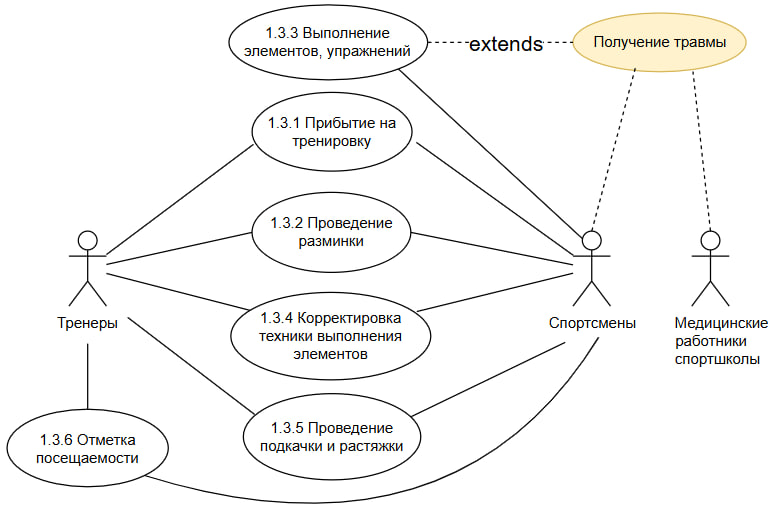
\includegraphics[width=1.0\linewidth]{images/6}
	\caption{Use-case диаграмма процесса проведения тренировок}
	\label{fig:im9}
\end{figure}	
\par \textbf{Акторы:} Спортсмены, тренеры, медицинские работники спортшколы.
\par \textbf{Триггер:} Начало учебно-тренировочного сезона.
\par \textbf{Входные данные:} Расписание тренировок, сформированные списки учебных групп, медицинские допуски спортсменов.
\par \textbf{Выходные данные:} Улучшение физической подготовки спортсменов, статистика посещаемости.

\newpage
\par \textbf{Основной процесс:}
\begin{enumerate}[nosep, label=1.3.\arabic*]
	\item Спортсмены прибывают на тренировку в назначенное время.
	\item Тренер проводит разминку и основные тренировочные упражнения.
	\item Спортсмены выполняют упражнения под руководством тренера.
	\item Тренер корректирует технику выполнения упражнений.
	\item Тренер проводит завершающую часть тренировки (подкачка и растяжка).
	\item Тренер ведет статистику посещаемости спортсменов.
	\item Переход к п. 1.3.1.
\end{enumerate}

\par \textbf{Альтернативный процесс:} \\
1.3.1.1 Пропуск тренировки без уважительной причины. Тогда тренер проводит беседу с родителями. \\
1.3.3.1 Получение травмы. Медицинские работники спортшколы оказывают первую помощь спортсмену.\\

\subsubsection{Use-case 1.5}
\par На \hyperref[fig:im10]{рисунке 10} представлена use-case диаграмма процесса присвоения спортивных разрядов. 
\begin{figure}[h!]
	\centering
	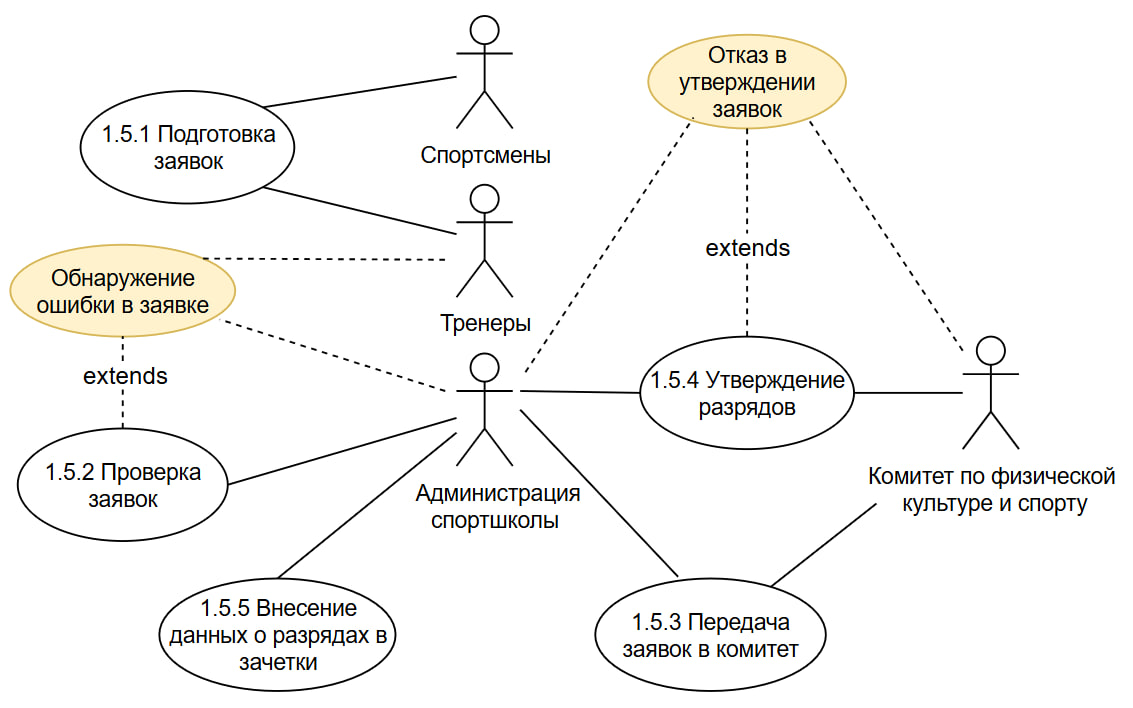
\includegraphics[width=1.0\linewidth]{images/7}
	\caption{Use-case диаграмма процесса присвоения спортивных разрядов}
	\label{fig:im10}
\end{figure}	

\par \textbf{Акторы:} Спортсмены, тренеры, администрация спортшколы, комитет по физической культуре и спорту.
\par \textbf{Триггер:} Достижение спортсменом необходимых нормативов.
\par \textbf{Входные данные:} Заявки на присвоение разрядов, протоколы соревнований.
\par \textbf{Выходные данные:} Присвоенные спортивные разряды, отказ в утверждении разрядов.

\par \textbf{Основной процесс:}
\begin{enumerate}[nosep, label=1.5.\arabic*]  
	\item Тренер подготавливает заявки на присвоение разрядов.
	\item Администрация спортшколы проверяет заявки.
	\item Администрация спортшколы направляет заявки в комитет по физической культуре и спорту.
	\item Комитет по физической культуре и спорту утверждает разряды.
	\item Администрация спортшколы вносит данные о разрядах в зачетные книжки спортсменов.
\end{enumerate}

\par \textbf{Альтернативный процесс:} \\
1.5.3.1 Обнаружение ошибки в заявке. Администрация спортшколы возвращает ее тренеру на доработку. \\
1.5.4.1 Отказ в утверждении разрядов. Комитет по физической культуре и спорту уведомляет администрацию спортивной школы о причинах отказа в утверждении разрядов. 

\subsection{Уровень 3}
\subsubsection{Use-case 1.1.1}
\par На \hyperref[fig:im11]{рисунке 11} представлена use-case диаграмма процесса подачи родителем заявки на зачисление детей в спортивную школу.
\begin{figure}[h!]
	\hspace{- 1.55cm} 
	\centering
	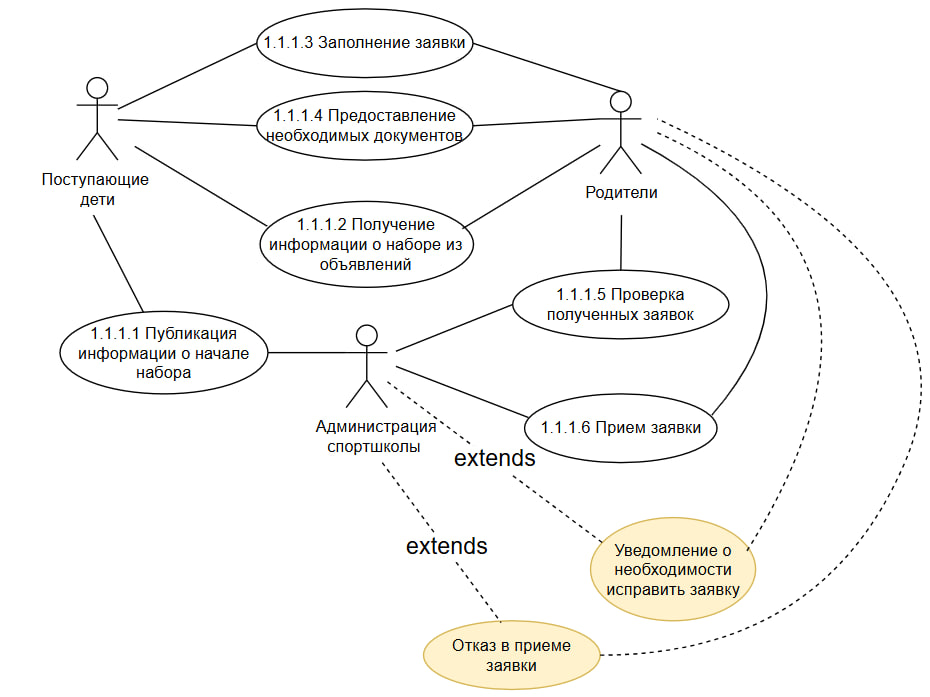
\includegraphics[width=0.9\linewidth]{images/8}
	\caption{Use-case диграмма процесса подачи родителем заявки на зачисление детей в спортивную школу}
	\label{fig:im11}
\end{figure}	

\par \textbf{Акторы:} Родители, администрация спортшколы, поступающие дети.
\par \textbf{Триггер:} Начало учебно-тренировочного сезона.
\par \textbf{Входные данные:} Объявление о наборе детей в спотшколу, желание родителей записать детей в спортивную школу.
\par \textbf{Выходные данные:} Заполненная заявка на зачисление, регистрация заявки в журнале поступающих, отклонение заявки с указанием причины.

\par \textbf{Основной процесс:}
\begin{enumerate}[nosep, label=1.1.1.\arabic*]
	\item Администрация спортшколы публикует информацию о начале набора;
	\item Родители получают информацию из объявлений;
	\item Родители заполняют заявку;
	\item Родители прилагают к заявке копии документов;
	\item Администрация проверяет полученные заявки;
	\item Администрация сообщает родителям о принятии заявки и дальнейших действиях. 
\end{enumerate}

\par \textbf{Альтернативный процесс:} \\
1.1.1.6.1 Неполное заполнение заявки. Администрация спортшколы сообщает родителям о необходимости исправить заявку или донести документы до заданного срока. \\
1.1.1.6.2 Медицинские противопоказания. Если в справке указаны заболевания/ограничения, несовместимые с выбранным спортом, администрация выдает письменный отказ приема заявки с указанием причины.

\newpage
\section{BPM}
\subsection{BPM-диаграмма для Use-case 1.1}
\par BRM-диаграмма процесса набора детей в спортшколу представлена на рисунке 12.

\subsection{BPM-диаграмма процесса бронирования гостиницы для выездных соревнований}
\par BRM-диаграмма процесса бронирования гостиницы для выездных соревнований представлена на рисунке 13.

\newpage
\includepdf[pages=-,fitpaper]{bpm1.pdf} 

\newpage
\includepdf[pages=-,fitpaper]{bpm2.pdf} 
\setcounter{figure}{13}



\end{document}